\chapter{A Genetic Ant Colony Optimization Algorithm for Inter-domain Path Computation problem under the Domain Uniqueness constraint}
\label{chap:chap3}
This section introduces the proposed two-level genetic ant colony optimization algorithm, called \acrshort{gaco} hereafter, to solve \gls{idpcdu} in more detail. Each level in \acrshort{gaco} is responsible for a separate task, where the first level establishes the domains' priorities, which are then used as input for the second one to find the final solution. The structure of \acrshort{gaco} is presented in Figure~\ref{fig:flowchart}.

\setlength{\intextsep}{3pt}
\renewcommand{\scalefigure}{0.85}
\begin{figure}[htbp]
	\centering
	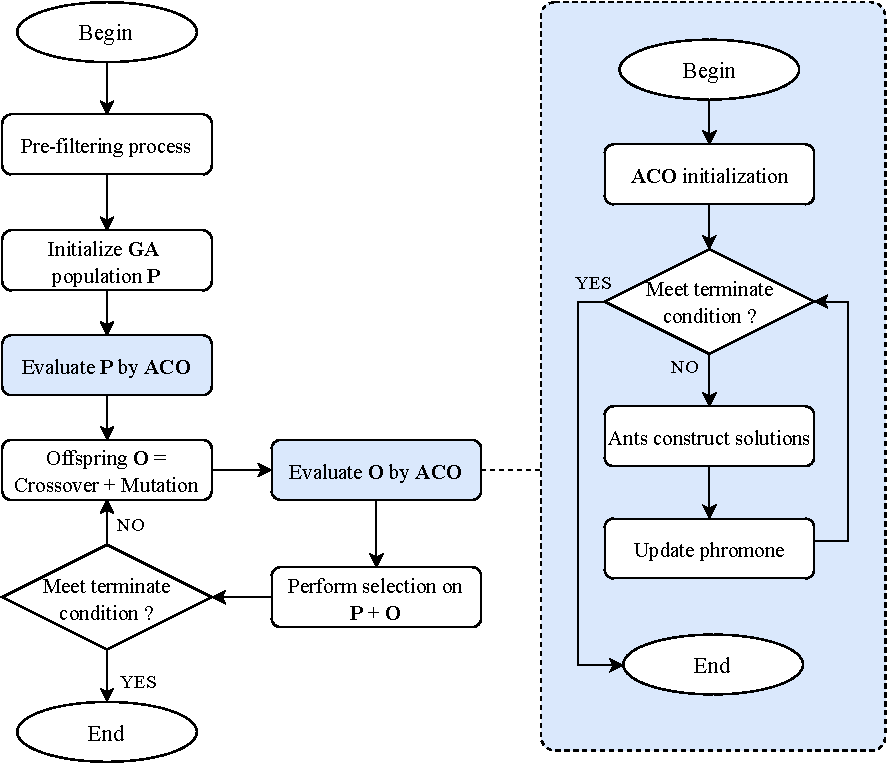
\includegraphics[scale=\scalefigure]{Figures/chap 3/Flowchart.pdf}
	\caption{The structure of \acrshort{gaco}}
	\label{fig:flowchart}
\end{figure}

\section{Pre-filtering Process}
\label{proposed:prefiltering}
Clearly, \gls{idpcdu}'s primary goal is to locate the minimally costly path. Therefore, to accelerate the search process and reduce resource consumption as well as computation time, a pre-filtering process, based on~\cite{binh2021two}, is applied to the input graph $G$ as follows. Firstly, we prune all edges that enter the source node $s$ and leave the target node $t$. Secondly, let $D^k_{i,j}$ be the set of $k$-colored edges going from node $i$ to $j$. If the length of $D^k_{i,j}$ is greater than one, we preserve only the lowest-weight edge and remove the remaining ones in $D^k_{i,j}$. Finally, apart from the source $s$ and target $t$, any node whose indegree and outdegree is 0, is likewise eliminated from $V$. Figure~\ref{fig:filtered_graph} demonstrates $G'=(E', V')$ as a result after performing the pre-filtering process on the input graph.

\setlength{\intextsep}{3pt}
\renewcommand{\scalefigure}{0.8}
\begin{figure}[htbp]
	\centering
	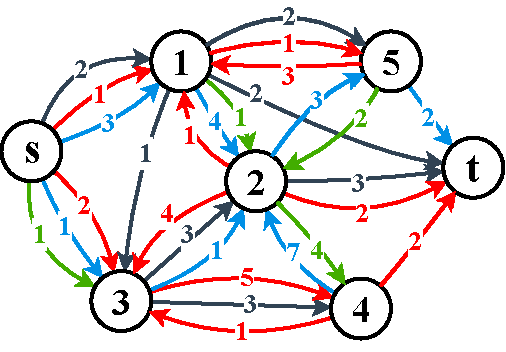
\includegraphics[scale=\scalefigure]{Figures/chap 3/Bold Filtered Graph.pdf}
	\caption{The filtered graph $G'$}
	\label{fig:filtered_graph}
\end{figure}

\section{Individual Representation}
\label{proposed:encoding}
This section introduces a scheme to represent a solution of \gls{idpcdu} as an individual in \gls{ea}. In general, for a difficult problem, significant advantages may be gained by an effective encoding method. Instead of conventional path encoding approach (such as representing a path from $s$ to $t$ with a list of edges/nodes between them), each chromosome is constructed by an array of real numbers whose length is equal to the number of domains. Each element, which denotes the priority of each domain, is randomly drawn between 0 and 1. The higher the priority value, the earlier the domain is likely to be visited. Each chromosome is then evaluated by an improved \gls{aco} algorithm, where the domain's priority will act as a factor influencing the ant's route selection. This encoding helps with facilitating the evolution operators by ensuring all chromosomes' length is equal. Furthermore, in many practical cases, the number of domains is remarkably smaller than the number of nodes or edges. 
Figure~\ref{fig:individual} delineates an example of an individual representation, in which the priority values of each domain are $red - 0.8$, $blue - 0.2$, $green - 0.6$, and $grey - 0.3$, respectively.
\setlength{\intextsep}{3pt}
\renewcommand{\scalefigure}{1.2}
\begin{figure}[htbp]
	\centering
	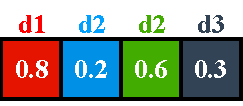
\includegraphics[scale=\scalefigure]{Figures/chap 3/Individual.pdf}
	\caption{A representation of a chromosome}
	\label{fig:individual}
\end{figure}

\section{Evolutionary Operators}
\label{proposed:operator}
\subsection{Crossover}
Since the proposed encoding utilizes an array of real numbers, this thesis apply the \gls{sbx}~\cite{deb1995simulated}. \gls{sbx} has been applied in many real-coded \gls{ga} problems and it also has proven to be effective. The implementation steps of \gls{sbx} can be summarized as follows. Firstly, choose a random number $u = [ \, 0, 1) \,$. Next, the ratio of the difference in offspring values to their parents' values $\beta$ is calculated as:
\begin{equation}
	\beta = 
	\begin{cases}
		(2u)^{\frac{1}{\eta_c + 1}}, & \text{if $u \leq 0.5$},\\
		(\frac{1}{2(1 - u)})^{\frac{1}{\eta_c + 1}}, & \text{otherwise},
	\end{cases}  
\end{equation}
where $\eta_c$ is any non-negative real number indicating the distribution index. A large value of $\eta_c$ increases the likelihood of generating near-parent solutions, whereas a small one allows for the selection of distant solutions as children. Finally, for two parents $p_1$ and $p_2$, two offspring $o_1$ and $o_2$ are reproduced using:
\begin{equation}
	o^i_1 = 0.5*[(1-\beta)*p^i_1 + (1+\beta)*p^i_2],
\end{equation}
\begin{equation}
	o^i_2 = 0.5*[(1+\beta)*p^i_1 + (1-\beta)*p^i_2].
\end{equation}

\subsection{Mutation}
In like manner, this thesis use \gls{pm}~\cite{deb2014analysing}, which is also an operator used in real-coded \gls{ga}. From a selected parent $p$, the \gls{pm} produces an individual $p'$ as follows. Similar to \gls{sbx}, a random number $u = 	[ \, 0, 1) \,$ is picked at first. For each element $p_i$, the $\delta_i$ is calculated as:
\begin{equation}
	\delta_i = 
	\begin{cases}
		(2u)^{\frac{1}{\eta_m + 1}} - 1, & \text{if $u \leq 0.5$},\\
		1 - [2(1-u)]^{\frac{1}{\eta_m + 1}}, & \text{otherwise},
	\end{cases}
\end{equation}
where $\eta_m$ is any non-negative real number indicating the polynomial distribution index. The perturbance can be varied in the mutated solution by changing $\eta_m$ value. $p'$ is then updated using the following equation:
\begin{equation}
	p' = 
	\begin{cases}
		p + \delta_i * p, & \text{if $u \leq 0.5$},\\
		p + \delta_i * (1-p), & \text{otherwise},
	\end{cases}
\end{equation}

\subsection{Selection}
Roulette Selection is used for selecting parents.

\section{Proposed Ant Colony Optimization as Fitness Evaluation}
\label{proposed:aco}
Corresponding to each chromosome, an improved \gls{aco} algorithm that plays the fitness evaluation role as well as finds the shortest path from the source node to the target node is proposed. 
To travel from node $v_i$, the $k^{th}$ ant must choose an edge $e$ in the $Adj(v_i)$ through a transition probability function (Equation~\ref{equation:edge_pick}).
\begin{equation}
	\label{equation:edge_pick}
	p_e(t) = 
	\frac{[\tau_e(t)]^{\alpha} \cdot [\eta_e(t)]^{\beta} \cdot  [P_e(t)]^{\gamma}}{\Sigma_{h \in Adj(v_i)} [\tau_h(t)]^{\alpha} \cdot [\eta_h(t)]^{\beta} \cdot [P_h(t)]^{\gamma}},
\end{equation}
where $P_e$ is the domain's priority of edge $e$ obtained from the input chromosome, and $\gamma$ is a constant representing the importance of this domain's priority value over the pheromone trail and ant's experience.

As can be seen, the difference between the probability function of the proposed algorithm and Equation~\ref{eq:aco_transition} lies in $P_e$. Based on this value, the ant will be navigated to select edges by their domain priority instead of random probability selection, which makes it difficult to fulfill the \gls{du}. The process of an ant finding the destination is described in Algorithm~\ref{alg:apa}.
\bigskip
\setlength{\intextsep}{3pt}
\renewcommand{\scalefigure}{1.1}
\begin{figure}[htbp]
	\centering
	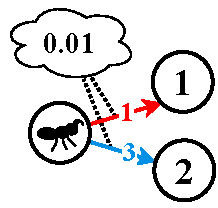
\includegraphics[scale=\scalefigure]{Figures/chap 3/pACO.pdf}
	\caption{An example of an ant find the next move}
	\label{fig:pACO}
\end{figure}

Take the instance in Figure~\ref{fig:individual} as an illustration input of the lower level. Suppose there is an ant that is finding its way to the next node as shown in Figure~\ref{fig:pACO}. In this case, the ant will have to choose one of two paths with the same pheromone trail of 0.01. Therefore, two main factors affecting the ant's path selection include the edge weight and the domain priority of that edge. Assume that the $\alpha, \beta,$ and $\gamma$ are 2, 1, and 2, respectively. The ant will now compute the $P_e$ value of each edge as follows.

\bigskip
$
p_e~red~edge = \frac{0.01^2~\times~(1/1)^1~\times~0.8^2}{(0.01^2~\times~(1/1)^1~\times~0.8^2)~+~(0.01^2~\times~(1/3)^1~\times~0.2^2)} = \frac{48}{49}~\approx0.97
$
\bigskip

$
p_e~blue~edge = \frac{0.01^2~\times~(1/3)^1~\times~0.2^2}{(0.01^2~\times~(1/1)^1~\times~0.8^2)~+~(0.01^2~\times~(1/3)^1~\times~0.2^2)} = \frac{1}{49}~\approx0.02
$ \\ 

It can be seen that the red edge has a higher ant selection rate (0.97 $>$ 0.02) due to its shorter path length and higher domain priority than the blue edge. In this step, Roulette Selection is implemented. Therefore, edges with a low selection rate can still be chosen by ants, which increases the exploitation capability of the colony and avoids falling into the local optima.

\begin{algorithm}
	%\setstretch{0.9}
	\caption{Ant's Pathfinding Algorithm (APA)}
	\label{alg:apa}
	\textbf{Input}:	
	\begin{itemize}
		\item A filtered multi-graph $G' = (V', E', w, s, t)$;
		\item An individual $I = (\pi_1, \pi_2,...,\pi_{|D|})$;
	\end{itemize}
	\textbf{Output}: A path $p = \{s, p_1, \dots, t\}$ and its cost. \\
	\Begin
	{	
		$D_{visited} \leftarrow\emptyset$ \Comment{List of visited domains}\;
		$visited[v] \leftarrow false~\forall v \in V$ \Comment{List of visited nodes}\;
		$cur \leftarrow s$ \Comment{The node that ant $k$ is visiting}\;
		$d \leftarrow  -1$ \Comment{The edge's domain that $p$ is visiting}\;
		\tcc{c(v) is the cost from s to v}
		$c(s) \leftarrow 0$, $c(t) \leftarrow \infty$;\\
		\While{$cur \neq t$}
		{
			$visited[cur] \leftarrow true$\;
			$Adj(cur) \leftarrow$ The set of edges that connect $v$ to other unvisited nodes in $G'$, in which each edge must satisfy the $Checksum$, $Domain~Blacklist~Check$, and its domain is not in $D_{visited}$\;
			%			$Adj(cur) \leftarrow$ Construct set of candidate edges 
			% \Comment{Refer to Algorithm~\ref{alg:edge-set}}\;
			\If{$Adj(cur) = \emptyset$}{ break\;}
			\If{$k$ is dull ant}{
				$e \leftarrow$ Choose an edge based on its attractiveness\;
			}
			\Else{
				Calculate the probability of moving to each edge as Equation (1)\;
				$e \leftarrow$ Choose an edge by $Roulette~Selection$\;
			}
			$d' \leftarrow$ the domain of $e$\;
			\If{$d \neq -1~and~d' \neq d$}{
				$D_{visited} \leftarrow D_{visited} \cup \{d\}$
			}
			$d \leftarrow d'$; $c(v) \leftarrow c(cur) + w(e)$;  $cur \leftarrow v$\; 
		}
		\Return $p$ and $c(t)$\;
	}
\end{algorithm}

In addition, to facilitate the ants’ search process and help ants avoid getting stuck, three components are integrated into the proposed \acrshort{gaco}, which will be discussed in the following subsections.

\subsection{Ant Colony Optimization with Dull Ants}
Typically, traditional \gls{aco} approaches have a potential drawback of premature convergence to a local optimum, often caused by a large amount of pheromone deposited by previous ant generations. Together with minimizing the impact of this phenomenon, a new type of ant, called $dull~ant$~\cite{shimomura2010ant}, is added to the colony. The notable feature of dull ant is that while it can neither trail the pheromone nor perceive the domains' priority, it can still deposit the pheromone. Therefore, dull ants will not be affected by other ants, opening up opportunities to discover alternatively better paths.

\subsection{Checksum}
To ease the search for each ant, a second component is employed, coined $Checksum$. Before choosing an edge $e$, ant $k$ will sum its current path length and the weight of $e$. If this sum is greater than the currently found best solution, $e$ is removed from the candidate edge set. Checksum not only expedites the ant's search process but also ensures that the solution located will always be better than the previous one.
Figure~\ref{fig:checksum} is a typical example of an ant checking the Checksum. Assume that the currently best solution found is 20 and the current path length of the considered ant is 17, and the \gls{du} are still satisfied.The ant will then sum its path value with each edge leading to the subsequent nodes. Following Checksum, the green edge leading to node 4 will be removed from the candidate edge set since $17 + 4 = 21 > 20$.

\setlength{\intextsep}{3pt}
\renewcommand{\scalefigure}{1.1}
\begin{figure}[htbp]
	\centering
	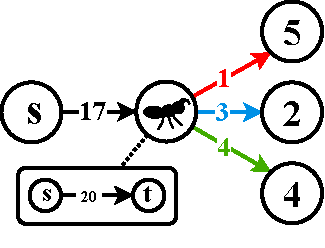
\includegraphics[scale=\scalefigure]{Figures/chap 3/CheckSum.pdf}
	\caption{An example of an ant checking the Checksum}
	\label{fig:checksum}
\end{figure}

\subsection{Blacklist of Domains on each Node}
One problem encountered when applying \gls{aco} to incomplete graphs is that ant gets stuck at a specific node since there is no subsequent path. Moreover, this phenomenon transpires more frequently in \gls{idpcdu}, where ant not only finds a path, but the path must also fulfill the \gls{du} constraint. In other words, a domain sequence is deemed to be stuck when an ant is unable to find any edges satisfying the \gls{du} constraint leading to one of the subsequent nodes. To remedy this shortcoming, an anti-stuck strategy for multi-domain problems like \gls{idpcdu} is proposed as follows. Except for the source and destination, every time an ant arrives at a stuck node, its list of visited domains is stored in the node's blacklist. Before deciding an edge $e$, the ant checks if the edge's domain $d$ is the one that causes a stuck of any sequence of domains in the blacklist of the node to which it leads. In such a case, the ant will continue to scan whether its list of visited domains is a superset of the other after discarding $d$. Consequently, $d$ will be removed from the candidate edge set if this point is satisfied. Algorithm~\ref{alg:blacklist} presents how to check if a list of domains is in the blacklist of any node. Note that before being saved to the blacklist as well as when the ant performs the $Domain~Blacklist~Check$, the domains will be sorted in a particular predefined order. Thus, the retrieval of data is performed faster, saving both time and resources.

\bigskip
\begin{algorithm}
	%\setstretch{0.9}
	\caption{Domain Blacklist Check}
	\label{alg:blacklist}
	\textbf{Input}:	
	\begin{itemize}
		\item A list of domains $LD$;\\
		\item A blacklist $blacklist^v$ of node $v$;\\
	\end{itemize}
	\textbf{Output}: $LD$ is in $blacklist^v$ or not.\\
	\Begin
	{	
		$d \leftarrow $ the last element in $LD$\;
		$LD' \leftarrow LD$ without $d$\;		
		\ForEach{list of domains $LD_i$ in $blacklist^v$}
		{
			$d_i \leftarrow $ the last element in $LD_i$\;
			\If{$d = d_i$}
			{
				$LD_i' \leftarrow LD_i$ without $d_i$\;
				\If{$LD_i' \subseteq LD'$} {\Return true\;}
			}
		}
		\Return false\;
	}
\end{algorithm}
\bigskip
\setlength{\intextsep}{3pt}
\renewcommand{\scalefigure}{1}
\begin{figure}[htbp]
	\centering
	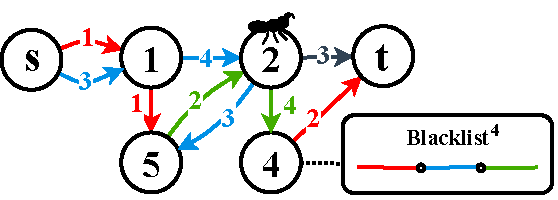
\includegraphics[scale=\scalefigure]{Figures/chap 3/BlacklistV2.pdf}
	\caption{An example of an ant checking the blacklist}
	\label{fig:blacklist}
\end{figure}
\bigskip
Take Figure~\ref{fig:blacklist} as a sample blacklist implementation in ant's route selection. Suppose that the blacklists of all nodes are initially empty, and an edge that goes from node $i$ to $j$ with an associated weight $w$ and belongs to domain $d$ is denoted by $(i, j, w, d)$. The first ant starts from $(s, 1, 1, red)$, $(1, 2, 4, blue)$, $(2, 4, 4, green)$ and gets stuck at node 4 because it can only revisit the $red$ domain. Therefore, the order of domains $(red, blue, green)$ is added to the blacklist of node 4. The next ant has the same beginning as the previous one. When standing at node 2, it realizes that there is only one route $(2, 4, 4, green)$, which also belongs to the domain that caused the stuck at node 4. The ant then resumes checking and finds that its visited domains list is also the stuck list without the $green$ domain. Therefore, the ant will remove this edge from the candidate set and select another. An ant has the following path $(s, 1, 3, blue)$, $(1, 5, 1, red)$, $(5, 2, 2, green)$. When it reaches node 2, it does the same thing as the second ant. In this case, its traversed domains list is a superset of the one after discarding the $green$ domain, and in the end, the edge $(2, 4, 4, green)$ is still eliminated. This strategy allows the searching candidate edge of ant more thoroughly without saving a plethora of stuck cases. The shorter the order of domains in blacklists, the more effective this method will be.

\section{Node-defined Domain - A variant of IDPC-DU}
\label{proposed:ndu}
As mentioned above, \acrshort{idpcndu}, which has also been proven to be NP-complete~\cite{maggi2018domain}, is a variant of the original \gls{idpcdu}. In general, previous approaches for \gls{idpcdu} or \acrshort{idpcndu} are often unable, or they have to go through several transformation steps to solve the remaining one. Our proposed algorithm, on the other hand, can be applied to both problems. Since \acrshort{idpcndu} no longer assigns domains on edges, there is only one edge with the smallest weight between any two nodes~\cite{binh2021two}. Therefore, $P_e$ in Equation~\ref{equation:edge_pick} is the domain's priority of the node to which edge $e$ leads. $Adj(v_i)$ now includes all nodes that ant $k$ has not yet traversed, whose domains satisfy the \gls{du} and $Domain~Blacklist~Check$, and the edges directing to these nodes fulfill the $Checksum$.